\section{Overall description}

\subsection{Product perspective}
	
	The product is not independent nor totally self-contained but defines a component of a larger system. This subsection relates the requirements of that larger system to functionality of the software and identifies interfaces between that system and the software.
	
	A class diagram in UML that describes the general structure of the system showing the system's classes, their attributes, operations (or methods), and the relationships among objects is represented in \autoref{fig:classDiagram}. To ensure a better readability not all class attributes and operations are represented. \newline \newline
		
	\begin{figure}[h]
			\centering
			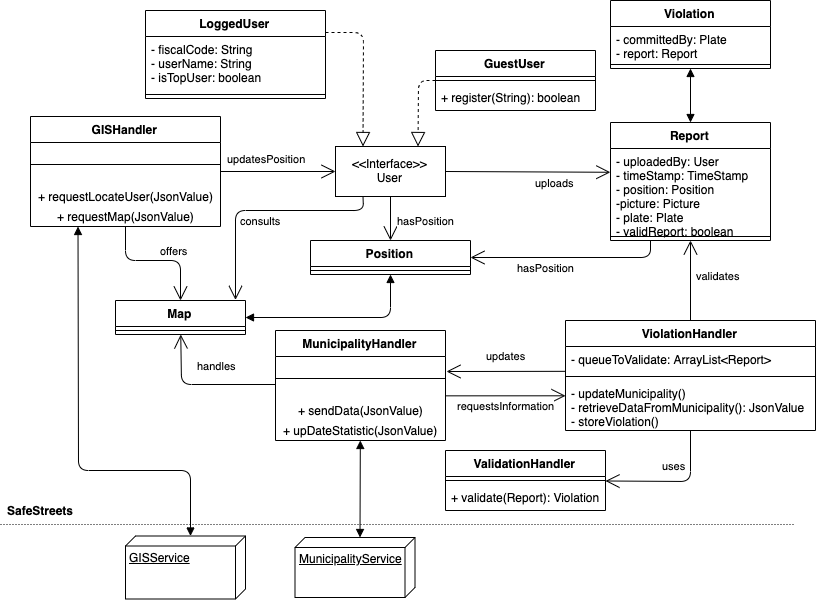
\includegraphics[width=350pt]{uml.png}
			\caption{
				\label{fig:classDiagram} 
				Class Diagram
			}
		\end{figure}

	\subsubsection{System interfaces}
	\label{sec:systemInterfaces}
		The system requires some external interfaces (represented in \autoref{fig:systemInterfaces}) to accomplish the \hyperref[sec:goals]{goals stated before}. \newline \newline
		\begin{figure}[h]
			\centering
			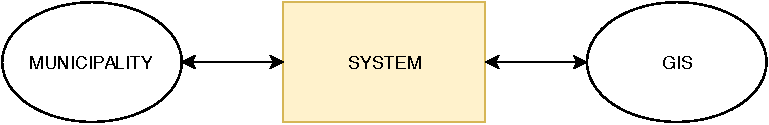
\includegraphics[width=300pt, height=50pt]{system_blocks}
			\caption{
				\label{fig:systemInterfaces} 
				Overview of system interfaces
			}
		\end{figure} 
\clearpage			
\paragraph{Municipality Data Exchange} The system will interact with municipalities. The system will retrieve the information about the accidents that occur on the territory of the municipality and cross this information with its own data to identify potentially unsafe areas. It will also retrieve the information about issued tickets from the municipalities to build statistics, for example about the most egregious offenders, or the effectiveness of the SafeStreets initiative (e.g., by looking for trends in the issuing of tickets). In addition, our system will expose via a \emph{restricted access API} the stored information about the violations to the municipalities, so that the local authorities can generate traffic tickets from it, and receive suggestions for possible interventions (e.g., add a barrier between the bike lane and the part of the road for motorised vehicles to prevent unsafe parking). 
		
\paragraph{Geographic Information System} The system will interact with an external GIS. Our system will map the spatial location of stored violations and visualise the spatial relationships among them. The external GIS will map quantities, such as where the most and least number of violations occurred, to find places that meet the user requested criteria inside an area of interest. This can be accomplished mapping concentrations, or a quantity normalised by area or total number. The system can map the change in a specific geographic area to visualise statistics, or to evaluate the results of the SafeStreets initiative.	

\subsubsection{User interfaces}

The system requires a user interface as the access point where users interact with the system. As the user interface design can dramatically affect the usability and user experience of the system, the layout of the user interface will be clearly set out so that elements can be found in a logical position, in a way that users will be able to find the the information and services they are looking for.

\paragraph{Guest user}
	Using the user interfaces of the system guest users can:
	\begin{itemize}
		\item Register to the system
		\item Authenticate and log-in to the system
	\end{itemize}
	
\paragraph{Logged User}
	Using the user interfaces of the system logged users can:
	\begin{itemize}
		\item Submit a violation with all the required and optional metadata
		\item View a map through an external GIS with highlighted streets (or areas) with the highest frequency of violations
		\item View statistics on vehicles that commit the most violations, the most egregious offenders, or the effectiveness of the SafeStreets initiative.
		\item View and edit personal information
	\end{itemize}
		
\subsubsection{Hardware interfaces}
	The system will interact with the user's device hardware interfaces.	
	\begin{itemize} 
		\item Telephony and other wireless connections are leveraged for the communication between the user and the system
		\item Full access to the user's device camera hardware is needed for the user to capture a photo
		\item The geomagnetic field sensor and the proximity hardware-based sensor are leveraged to determine the position of the user's device
	\end{itemize}

\subsubsection{Software interfaces}
	In order to reach the goals highlighted in the goals section the system requires to interface with Databases and DBMSs, required in order to store data about users, violations, and the corresponding metadata. These interfaces are also required to guarantee the ability to input queries to the database in order to satisfy the system required capabilities.
	
\subsubsection{Communication interfaces}
	The system requires secure communication within the involved entities in a way not susceptible to eavesdropping or interception. Secure communication includes means by which the system can share information that third parties cannot intercept or alter. For these reasons communication encryption methods must be implemented in a way that guarantees the use of encryption, i.e. if encrypted communication is impossible then no traffic is sent.

\subsection{Product functions}
\paragraph{Violation upload procedure} 
Provide logged users with the possibility to notify authorities when traffic violations occur and, in particular, parking violations. The application allows users to send pictures of violations, including suitable metadata.
SafeStreets then stores the information provided, completing it with suitable meta-­data. In particular, when it receives a picture, it runs an algorithm to read the license plate number (the user can help with the recognition) and it stores the retrieved information with the violation, including also the type of the violation (submitted by the user) and the name of the street where the violation occurred.

\clearpage

	\begin{figure}[h]
		\centering
		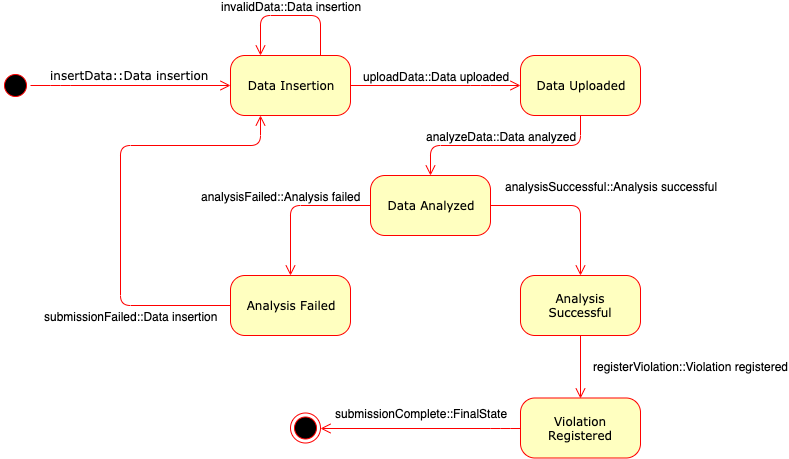
\includegraphics[width=320pt]{SubmitViolation.png}
		\caption{
			\label{fig:violationUpload} Violation upload process
		}
	\end{figure}
	
\paragraph{Retrieve data from municipality}
Retrieve the information about the accidents that occur on the territory using the service offered by the municipalities and cross these data with SafeStreets data, to identify potentially unsafe areas. This will also allow the system to understand which violations are more likely to cause accidents in a particular zone and elaborate suggestions on possible interventions, later communicated to the municipality via a \emph{restricted access API} provided to them. \newline
	\begin{figure}[h]
		\centering
		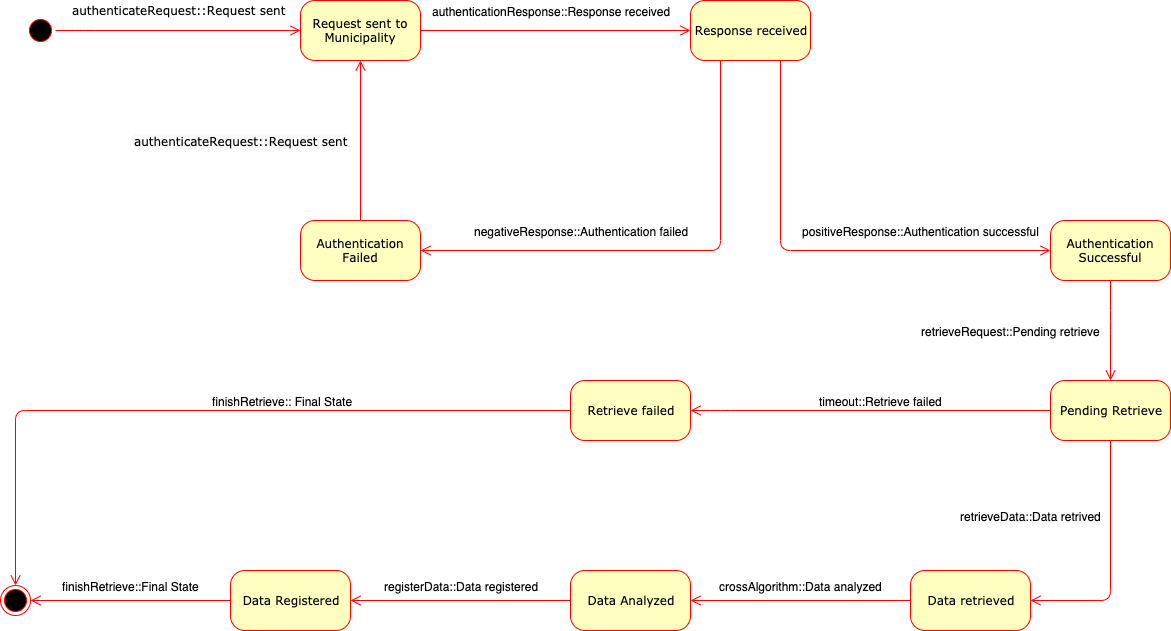
\includegraphics[width=285pt,height=205pt]{RequestMunicipality.png}
		\caption{
			\label{fig:retrieveMunicipality} Retrieve data from municipality
		}
	\end{figure}
	
\clearpage

\paragraph{Show information and statistics}
The application allows logged users to mine the information that has been received, highlighting the streets (or the areas) with the highest frequency of violations, considered unsafe areas, or the vehicles that commit the most violations. In addition, statistics about issued tickets, for example about the most egregious offenders, or the effectiveness of the SafeStreets initiative, are shown to the user if requested. 
	\newline
	\begin{figure}[h]
		\centering
		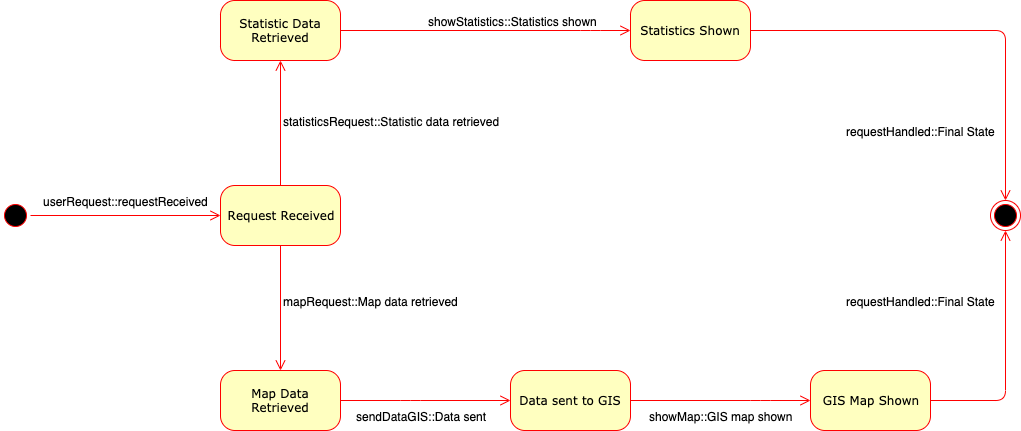
\includegraphics[width=310pt, height=145pt]{ShowStatistics.png}
		\caption{
			\label{fig:showStatistics} Show information and statistics
		}
	\end{figure}
	
\paragraph{Restricted access API}
The system will expose via a \emph{restricted access API} the stored information about the violations to the municipalities, so that the local authorities can generate traffic tickets from it and receive suggestions for possible interventions to carry out (e.g., add a barrier between the bike lane and the part of the road for motorised vehicles to prevent unsafe parking), in order to decrease the risk of those areas, so increasing their safety. 
	\newline
	\begin{figure}[h]
		\centering
		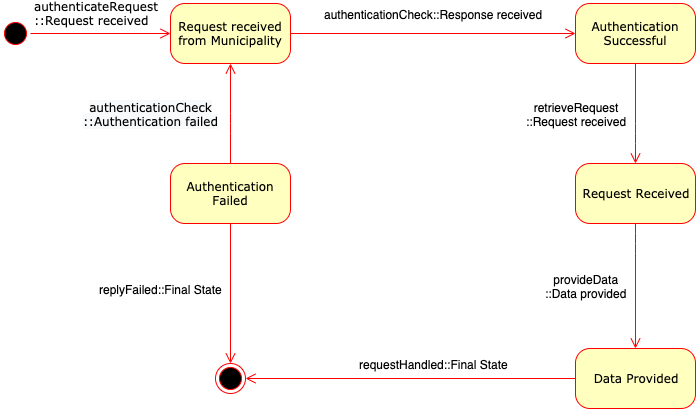
\includegraphics[width=315pt, height=185pt]{RequestAPI.png}
		\caption{
			\label{fig:restrictedAPI} Restricted access API
		}
	\end{figure}


\subsection{User Characteristics}
	Users can use our system when they notice a violation and want to communicate it to the authorities.\\
 	Necessary conditions for the user in order to use the system are:
 	\begin{itemize}
 		\item The user must have a smartphone with a working connection to the internet and he must be able to properly use it
 		\item The user must be in the age of majority
 		\item The user must be able to identify a violation and its type
 	\end{itemize}
 	The user agrees to these conditions during the registration to the system.
 	
\subsection{Constraints}
\label{sec:constraints}
	We assume that these constraints are always met:
	\begin{enumerate}[label=\textbf{C\arabic*}]
		\item GPS position is supposed to be accurate (max error $\pm5$m)
		\item The quality of the picture is sufficient to recognise the plate number (min resolution 320x240)
		\item Internet connection must be strong enough to allow the upload of the picture in a reasonable amount of time (supported technologies are 3G, 4G and 5G due to the performance requirement)
	\end{enumerate}
	
\subsection{Assumptions}
	We assume that these assumptions hold true in the domain of our system 
	\begin{enumerate}[label=\textbf{	DA\arabic*}]
		\item GPS position of all users is always obtainable
		\item Internet connection always works correctly
		\item Municipality services are always reachable
		\item The maps provided by the GIS are always reachable and up to date
		\item The DBMS always works properly so that the information in the DB are always accessible
		\item The smartphone of the user runs iOS (9 or later) or Android (Jelly Bean or later)
	\end{enumerate}
		
\clearpage